This thesis presents a number of novel approaches to the analysis of spike trains, the electrical signals which carry information throughout the brain. It has long been noted that different stimuli influence the rate at which neurons fire \citep{Knight1972a}, however, more recently it has been observed that stimuli can be encoded by the temporal precision of signals \citep{HopkinsBass1981a,EngelEtAl1992a}.
 
The advancement of computer processing power has led to increased analysis of the highly temporal data sets found in neuroscience. Computational neuroscience is a rapidly growing field of study which looks to apply the expertise of other branches of science and engineering to mine and model neuroscience data.  As a subset of computational neuroscience, mathematical neuroscience uses many different mathematical concepts to model the behaviour of the brain at many different levels.
 
The level of study which is of interest in this thesis is the bottom-most level of neural activity.  Rather than studying communication between different brain regions, spike train analysis focuses on the signals produced by single neurons.


\section{Spike trains}

There are many different types of neurons in the brain. In Figure \ref{Cajal} there are two such variations, as drawn and documented by \citet{Cajal1904a} in the late 19th and early 20th century. Pyramidal cells, for example, are abundant in the cerebrum cortex, and Purkinje cells are found in the cerebellum.  They have differing purposes in the nervous system, but they all accept and emit electrical signals to communicate with other neurons.

\begin{figure}
\begin{center}
\begin{tabular}{cc}
{\bf (a)} & {\bf (b)} \\
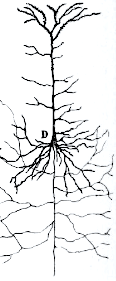
\includegraphics[width=1.6in]{CajalPyrD} & 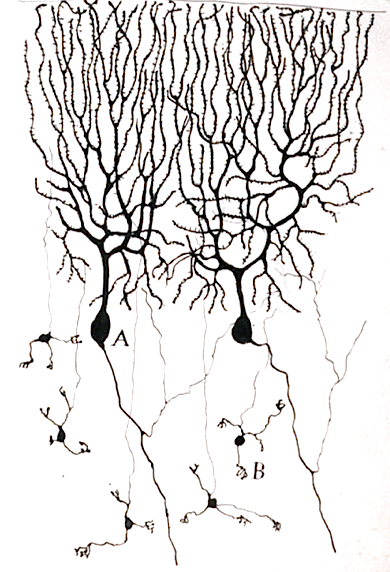
\includegraphics[width=2.62in]{CajalPurkinje}
\end{tabular}
\bigskip
\rule{33em}{0.5pt}
\caption{\label{Cajal} Diagrams of neurons as drawn by \citet{Cajal1904a}.  (a) depicts a cortical pyramidal cell .  Pyramidal cells are the primary excitatory neurons of the cerebral cortex.  Pyramidal cells are thus often modelled as a typical neuron.  (b) depicts a Purkinje cell of a pigeon.  Purkinje cells are found in the cerebellum in the human brain. They are some of the largest cells in the human brain. With their dense branching dendrites they have much higher connectivity than pyramidal cells.}
\end{center}
\end{figure} 

Neurons convey information through the nervous system by generating
electrical pulses which propagate along nerve fibers.  These pulses are
called action potentials or spikes, first observed in \citep{DuBoisReymond1884a}.  

A typical cortical pyramidal neuron has a resting potential of approximately -70 mV relative to
its surroundings, the cell is said to be polarised at this point.
The membrane potential of a neuron is changed by current
flowing into its synapses from other neurons, most of which make the membrane potential less negative, but the potential tends back towards the resting potential
unless it nears a certain threshold. If a neuron
is depolarised so that its membrane potential is raised above this
threshold, the neuron generates an action potential. An action potential, or 
spike, is a rapid depolarisation and repolarisation of the membrane potential.  Such a fluctuation in the membrane potential typically lasts 
approximately 1 ms. Following the production of a spike, the neuron briefly 
becomes hyperpolarised, that is, the potential drops to below its resting level. A neuron cannot generate a spike for several milliseconds after a spike. This period, when a spike cannot be fired, is
called the absolute refractory period of a neuron.  There is also a period in which
it is more difficult for the neuron to spike again, which is called
the relative refractory period. 

\begin{figure}[htb]
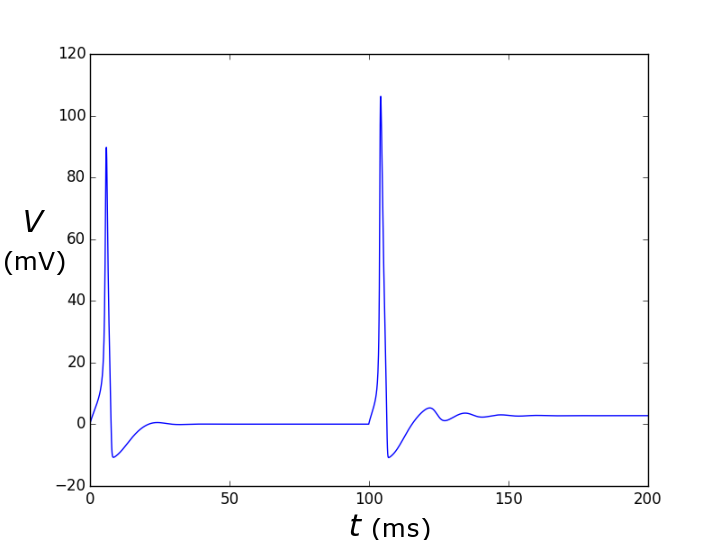
\includegraphics[width=\textwidth]{hhtrace}
\bigskip
\rule{33em}{0.5pt}
\caption{The voltage trace of a pair of spikes generated by the Hodgkin-Huxley model.  Simulation run using the python package Brian \citep{GoodmanBrette2008a}}
\end{figure}

The dynamics of the membrane potential were precisely modelled in \citep{HodgkinHuxley1952a} by modelling the flow of sodium and potassium ions into and out of the neuron.  Their model was based on the voltage traces that they recorded from the giant axon in a squid \citep{HodgkinHuxley1939a}. It has proven to be an excellent framework for biophysically accurate neuron models. The Hodgkin-Huxley models, with several currents to depict the flow of ions through the membrane, form the standard against which other neuron models are judged \citep{Izhikevich2004a}.

Spikes are very important to the study of communication in the brain, because they propagate over long distances without 
attenuation. Other sub-threshold fluctuations attenuate greatly over spaces as short as 1 mm. Therefore, spikes are the way in which neurons communicate with other regions 
throughout the nervous system.  While there is some variation in 
the duration, amplitude and shape of action potentials, for a single neuron they typically exhibit a characteristic voltage trace as discussed in \citep{Lewicki1998a}. The spike then can be represented by choosing a particular point of the typical action potential. Thus, the timing of the spikes give much of the information \citep{BiPoo1998a,Bair1999a}.  So, 
if a neuron spikes $n$ times in a certain trial, then the trial can be 
described by the timings of the spikes $t_i$.  The 
\emph{spike train} can then be described mathematically as:
\begin{equation}
X = x(t) = \sum_{i=1}^n \delta(t-t_i).
\end{equation}
The $\delta$ here is the Dirac delta function centred at $t_i$, which has a volume equal to 
one at the point $t_i$.

\section{Spike train metrics}

While observing spike trains from a specific neuron, ideally one would be able to 
\lq{}decode\rq{} them and be able to describe the stimulus which produced them.  
This problem is very difficult, particularly when looking at neurons \emph{in vivo}, that is, in living animals \citep{AverbeckEtAl2006a}. There tends to be a lot of noise from other neurons in the network which can obscure the signal to be reproduced \citep{Hopfield1982a}.  A first step which can be taken towards solving this problem is to try to distinguish which spike trains amongst a collection were share 
the same stimulus.  There are several \emph{metrics} in the 
literature which give a measure of the distance between pairs of spike trains.  

In Mathematics a metric space is a space equipped with a scalar function which gives a  
distance, of sorts, between two elements in the space.  The function is called a metric if it is a scalar function on a set 
$X$, $d: X\times X \rightarrow [0,\infty )$ that has the properties a distance might intuitively be expected to have. That is, distances are non-negative, 
symmetric and only zero if two elements are the same. The final property is called the triangle inequality, which is a rule that ensures the shortest 
distance between two points is a straight line.

\subsection{Victor-Purpura metric}

In \citep{VictorPurpura1997a} a family of metrics are described.  All the metrics are a type of metric called \lq{}edit-length\rq{} metrics. An edit-length metric is based on a theoretical \lq{}cost\rq{} of transforming one point in a space to another via elementary transformations.  The principle is that each transformation has a non-zero cost, so the distance between two spike trains can be measured by minimising  the cost to transform one spike train, $X$, into another, $Y$.

There are three different permitted fundamental transformations.  It is possible to insert a spike at any time, which has a cost of one.  Similarly, any spike can be deleted for a cost of one.  The third permitted transformation is to move a spike $\Delta t$, which has a cost $q\Delta t$, for some timescale parameter $q>0$.

The insertion and deletion operations may not appear to be influenced by the parameter $q$, but these operations do set a maximum cost of transformation from one spike to another at $2$.  Since a spike at any time can be deleted at a cost of one, and another inserted at a cost of one, this sets a maximum time-frame for transpositions at $2/q$.  Therefore, given two spikes, $t_a$ in $X$ and $t_b$ in $Y$:
\begin{equation}
c(f_i(t_a)) = \left\{ \begin{array}{ll} q | t_a - t_b | & | t_a - t_b | < 2/q \\ 2 & | t_a - t_b | \geq  2/q \end{array}\right.
\end{equation}\\
It follows that as $q$ tends towards zero, it becomes cheaper to move spikes than insert and delete them.  In that case, assuming there are more spikes in $Y$, the first $n$ spikes in $X$ would be transposed to match the times of the first $n$ spikes of $Y$.  Then the remaining spikes would need to be inserted at the remaining times.

Then the Victor-Purpura metric between two spike trains, $X$ and $Y$, is defined to be the minimum over all combinations of fundamental functions which transform $X$ to $Y$.  The metric can be written as:
\begin{equation}
d_{\text{VP}}(X,Y) = \min_f \sum_i c\left( f_i(X) \right)
\end{equation}
where $f=f_1\circ\ldots\circ f_m$ is a function such that $f(X) = Y$.

This is demonstrably a metric. There is a non-zero cost for each transformation, so $d(X,Y)=0$ only if $X=Y$. Due to the fact that insertion and deletion are symmetric with each other, and transposition is a symmetric operation, it is clear that $d(X,Y)=d(Y,X)$.  The triangle equality follows, since if $f$ transforms $X$ to $Y$, and $g$ transforms $Y$ to $Z$, then $h=g\circ f$ must transform $X$ to $Z$, and since the Victor-Purpura metric requires that the minimum cost, $h$ must have cost greater than or equal to $d(X,Z)$.

\subsection{van Rossum metric}

The metric proposed in 
\citep{VanRossum2001a}, is based on the $L^2$ metric on function 
spaces.  The $L^2$ metric between square integrable functions, $f,g$ , is the square root of the integral of the difference between $f$ and $g$ squared, that is:
\begin{equation}
\| f - g \|_2 = \int_0^{\infty} \sqrt{\left[ f(t)-g(t) \right]^2 }\, dt.
\end{equation}

\begin{figure}[htb]
% GNUPLOT: LaTeX picture with Postscript
\begingroup
  \makeatletter
  \providecommand\color[2][]{%
    \GenericError{(gnuplot) \space\space\space\@spaces}{%
      Package color not loaded in conjunction with
      terminal option `colourtext'%
    }{See the gnuplot documentation for explanation.%
    }{Either use 'blacktext' in gnuplot or load the package
      color.sty in LaTeX.}%
    \renewcommand\color[2][]{}%
  }%
  \providecommand\includegraphics[2][]{%
    \GenericError{(gnuplot) \space\space\space\@spaces}{%
      Package graphicx or graphics not loaded%
    }{See the gnuplot documentation for explanation.%
    }{The gnuplot epslatex terminal needs graphicx.sty or graphics.sty.}%
    \renewcommand\includegraphics[2][]{}%
  }%
  \providecommand\rotatebox[2]{#2}%
  \@ifundefined{ifGPcolor}{%
    \newif\ifGPcolor
    \GPcolorfalse
  }{}%
  \@ifundefined{ifGPblacktext}{%
    \newif\ifGPblacktext
    \GPblacktexttrue
  }{}%
  % define a \g@addto@macro without @ in the name:
  \let\gplgaddtomacro\g@addto@macro
  % define empty templates for all commands taking text:
  \gdef\gplbacktext{}%
  \gdef\gplfronttext{}%
  \makeatother
  \ifGPblacktext
    % no textcolor at all
    \def\colorrgb#1{}%
    \def\colorgray#1{}%
  \else
    % gray or color?
    \ifGPcolor
      \def\colorrgb#1{\color[rgb]{#1}}%
      \def\colorgray#1{\color[gray]{#1}}%
      \expandafter\def\csname LTw\endcsname{\color{white}}%
      \expandafter\def\csname LTb\endcsname{\color{black}}%
      \expandafter\def\csname LTa\endcsname{\color{black}}%
      \expandafter\def\csname LT0\endcsname{\color[rgb]{1,0,0}}%
      \expandafter\def\csname LT1\endcsname{\color[rgb]{0,1,0}}%
      \expandafter\def\csname LT2\endcsname{\color[rgb]{0,0,1}}%
      \expandafter\def\csname LT3\endcsname{\color[rgb]{1,0,1}}%
      \expandafter\def\csname LT4\endcsname{\color[rgb]{0,1,1}}%
      \expandafter\def\csname LT5\endcsname{\color[rgb]{1,1,0}}%
      \expandafter\def\csname LT6\endcsname{\color[rgb]{0,0,0}}%
      \expandafter\def\csname LT7\endcsname{\color[rgb]{1,0.3,0}}%
      \expandafter\def\csname LT8\endcsname{\color[rgb]{0.5,0.5,0.5}}%
    \else
      % gray
      \def\colorrgb#1{\color{black}}%
      \def\colorgray#1{\color[gray]{#1}}%
      \expandafter\def\csname LTw\endcsname{\color{white}}%
      \expandafter\def\csname LTb\endcsname{\color{black}}%
      \expandafter\def\csname LTa\endcsname{\color{black}}%
      \expandafter\def\csname LT0\endcsname{\color{black}}%
      \expandafter\def\csname LT1\endcsname{\color{black}}%
      \expandafter\def\csname LT2\endcsname{\color{black}}%
      \expandafter\def\csname LT3\endcsname{\color{black}}%
      \expandafter\def\csname LT4\endcsname{\color{black}}%
      \expandafter\def\csname LT5\endcsname{\color{black}}%
      \expandafter\def\csname LT6\endcsname{\color{black}}%
      \expandafter\def\csname LT7\endcsname{\color{black}}%
      \expandafter\def\csname LT8\endcsname{\color{black}}%
    \fi
  \fi
  \setlength{\unitlength}{0.0500bp}%
  \begin{picture}(7200.00,5040.00)%
    \gplgaddtomacro\gplbacktext{%
      \csname LTb\endcsname%
     % \put(462,3863){\makebox(0,0)[r]{\strut{} 0}}%
      %\put(462,4231){\makebox(0,0)[r]{\strut{} 1}}%
      %\put(462,4599){\makebox(0,0)[r]{\strut{} 2}}%
      \put(594,3580){\makebox(0,0){\strut{} 0}}%
      \put(1836,3580){\makebox(0,0){\strut{} 0.02}}%
      \put(3078,3580){\makebox(0,0){\strut{} 0.04}}%
      \put(4319,3580){\makebox(0,0){\strut{} 0.06}}%
      \put(5561,3580){\makebox(0,0){\strut{} 0.08}}%
      \put(6803,3580){\makebox(0,0){\strut{} 0.1}}%
      \put(3698,4929){\makebox(0,0){\strut{}(a)}}%
    }%
    \gplgaddtomacro\gplfronttext{%
    }%
    \gplgaddtomacro\gplbacktext{%
      \csname LTb\endcsname%
      \put(462,2183){\makebox(0,0)[r]{\strut{} 0}}%
      \put(462,2551){\makebox(0,0)[r]{\strut{} 1}}%
      \put(462,2919){\makebox(0,0)[r]{\strut{} 2}}%
      \put(594,1900){\makebox(0,0){\strut{} 0}}%
      \put(1836,1900){\makebox(0,0){\strut{} 0.02}}%
      \put(3078,1900){\makebox(0,0){\strut{} 0.04}}%
      \put(4319,1900){\makebox(0,0){\strut{} 0.06}}%
      \put(5561,1900){\makebox(0,0){\strut{} 0.08}}%
      \put(6803,1900){\makebox(0,0){\strut{} 0.1}}%
      \put(3698,3249){\makebox(0,0){\strut{}(b)}}%
    }%
    \gplgaddtomacro\gplfronttext{%
    }%
    \gplgaddtomacro\gplbacktext{%
      \csname LTb\endcsname%
      \put(462,503){\makebox(0,0)[r]{\strut{} 0}}%
      \put(462,749){\makebox(0,0)[r]{\strut{} 1}}%
      \put(462,994){\makebox(0,0)[r]{\strut{} 2}}%
      \put(462,1240){\makebox(0,0)[r]{\strut{} 3}}%
      \put(594,220){\makebox(0,0){\strut{} 0}}%
      \put(1836,220){\makebox(0,0){\strut{} 0.02}}%
      \put(3078,220){\makebox(0,0){\strut{} 0.04}}%
      \put(4319,220){\makebox(0,0){\strut{} 0.06}}%
      \put(5561,220){\makebox(0,0){\strut{} 0.08}}%
      \put(6803,220){\makebox(0,0){\strut{} 0.1}}%
      \put(3698,1570){\makebox(0,0){\strut{}(c)}}%
        \put(3698,10){\makebox(0,0){\strut{} $t$ (s)}}%
    }%
    \gplgaddtomacro\gplfronttext{%
    }%
    \gplbacktext
    \put(0,0){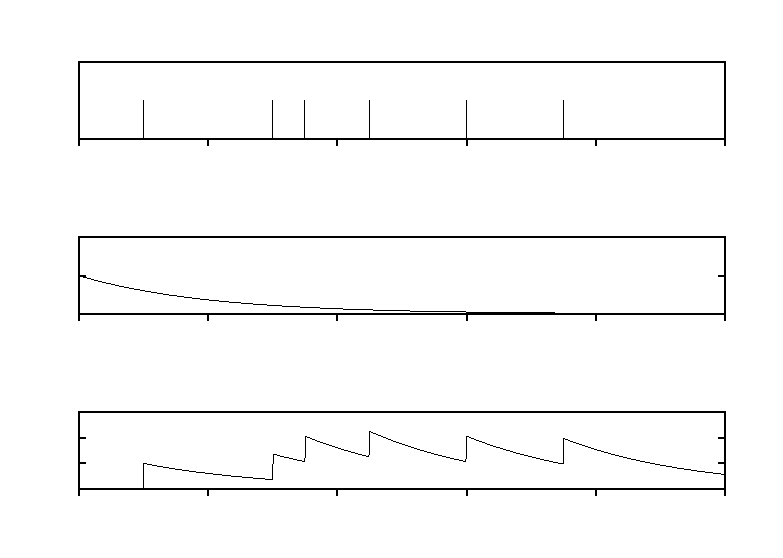
\includegraphics{vRfilter}}%
    \gplfronttext
  \end{picture}%
\endgroup

\bigskip
\rule{33em}{0.5pt}
\caption{\label{stk} Shown above is an example of the filtering process of the van Rossum metric.  {\bf (a)} A sample spike train is convolved with {\bf (b)} an exponential filter, where the timescale $\tau=20$ ms, to get {\bf (c)} the function $u(t)$ .}
\end{figure}

If spike trains are viewed as sums of Dirac delta functions, 
then by convolving the spike trains, $X=x(t)$, with 
a square-integrable kernel, $k(t)$, each spike train can be represented in an $L^2$ function space.  A common kernel is the exponential kernel as used in \citep{VanRossum2001a}:
\begin{equation}
k(t) = \left\{ \begin{array}{ll}\frac{1}{\tau}e^{-\frac{t}{\tau}}, & t\geq 0 \\
0, & t<0\end{array} \right. .
\end{equation}
this function is shown in Figure \ref{stk}.

This kernel has the potential advantage of causality over a 
Gaussian kernel, and it is very fast to calculate \citep{HoughtonKreuz2012a}.   Convolving the spike 
train with the kernel results in a function, $u(t)$, which is $L^2$ measurable:
\begin{equation}
u(t) = x*k(t) = \int_0^T x(t-s)k(s)\,ds
\end{equation}



%\begin{figure}[tb]
%  \centering
%  \includegraphics[width=0.8\textwidth]{spiketrainkernel.eps}
%  \rule{33em}{0.5pt}
%  \caption{This figure shows  an exponential kernel (a), which we convolve with a spike train (b), to get the function (c) which represents the spike train.  We take the  $L^2$-metric between such functions to get the van Rossum metric between spike trains.}
%  \label{stk}
%\end{figure}

Figure \ref{stk} shows the form of the function that is produced by
convolving a spike train with the exponential kernel.  The metric is then simply the $L_2$ distance between these functions:
\begin{equation}
d_{\text{vR}}(X,Y) =  \sqrt{\int_0^T (x*k(t) - y*k(t))^2\,dt}.
\end{equation}
It has been shown that once the correct timescale has been chosen the choice of kernel has 
little effect on the performance of this metric \citep{HoughtonVictor2009a}.

\subsection{ISI distance}
In \citep{KreuzEtAl2007a} a new type of measure was introduced.  The ISI distance is a time-local measure of spike train synchrony.  The ISI distance is defined for any $t$, $0<t<T$, in the trial.  The distance is a local comparison of the estimated firing rates of spike trains $X$ and $Y$.  

For any time $t$ in the trial, the firing rate of spike train $X$ is estimated by the reciprocal of the current inter-spike interval in $X$, and similarly for $Y$:
\begin{equation}
r_x(t) = \frac{1}{I_x(t)}, \hspace{20pt} r_y(t) = \frac{1}{I_y(t)}
\end{equation}
Typically one rate will be bigger than the other rate. Dividing by that rate a similarity measure, with values between zero and one, for the spike trains can be calculated:
\begin{equation}
s_{ISI}(X,Y)(t) = \left\{ \begin{array}{ll} r_x(t)/r_y(t) & ,r_y(t) \geq r_x(t)\\ r_y(t)/r_x(t) & , r_x(t) > r_y(t) \end{array}\right.
\end{equation}

\begin{figure}[hbt]
\begin{center}
\setlength{\unitlength}{.085cm}
\begin{picture}(140,65)
\put(3,9){\mbox{$\mathbf{Y}$}}
\put(3,39){\mbox{$\mathbf{X}$}}
\put(74.1,62.5){\mbox{$\mathbf{t}$}}
\linethickness{1pt}
\put(10,10){\line(1,0){130}}
\put(10,40){\line(1,0){130}}
\linethickness{0.5pt}
\put(25,10){\line(0,1){10}}
\put(50,10){\line(0,1){10}}
\put(100,10){\line(0,1){10}}
\put(130,10){\line(0,1){10}}
\put(20,40){\line(0,1){10}}
\put(60,40){\line(0,1){10}}
\put(120,40){\line(0,1){10}}
\put(135,40){\line(0,1){10}}
\linethickness{1.5pt}
\put(75,0){\line(0,1){9}}
\put(75,11){\line(0,1){3}}
%\put(75,16){\line(0,1){2}}
\put(75,22){\line(0,1){17}}
\put(75,41){\line(0,1){3}}
\put(75,46){\line(0,1){14}}
\linethickness{1pt}
\put(75,15){\vector(-1,0){25}}
\put(75,15){\vector(1,0){25}}
\put(90,45){\vector(-1,0){30}}
\put(90,45){\vector(1,0){30}}
\put(72.5,17.5){\mbox{$\mathbf{I_{y}(t)}$}}
\put(87.5,47.5){\mbox{$\mathbf{I_{x}(t)}$}}
\end{picture}
\bigskip
\rule{33em}{0.5pt}
\caption{\label{isiex} Shown here is an example pair of spike trains $X$ and $Y$.  At each point $t$ in the trial there are respective intervals $I_x(t)$ and $I_y(t)$. By taking the reciprocal of $I_x(t)$ and $I_y(t)$, an estimator for the firing rate of $X$ and $Y$ at time $t$ is calculated.}
\end{center}
\end{figure}

Since the rates are estimated by the ISIs, and $1/a \geq 1/b \implies a \leq b$, this can be rewritten as:
\begin{equation}
s_{ISI}(X,Y)(t) =  = \left\{ \begin{array}{ll} I_y(t)/I_x(t) & ,I_x(t) \geq I_y(t)\\ I_x(t)/I_y(t) & , I_y(t) > I_x(t) \end{array}\right.
\end{equation}

This similarity measure is always between zero and one, so to change it to a distance measure between spike trains, all that had to be done was to take it from one.  Then the ISI distance, as defined in \citep{KreuzEtAl2007a,KreuzEtAl2009a}, is:
\begin{equation}
d_{ISI}(X,Y)(t) = \left\{ \begin{array}{ll} 1 - \frac{I_y(t)}{I_x(t)} & ,\, I_x(t) \geq I_y(t) \\ 1 - \frac{I_x(t)}{I_y(t)} & ,\, I_y(t) > I_x(t) \end{array} \right.
\end{equation}
The ISI distance is zero when the inter-spike intervals of $X$ and $Y$ are the same, and tends towards one as the ratio between them increases.

The ISI distance was found to have a simpler form, which benefits the extension work of Chapter Three of this thesis, as it shows the nature of the ISI distance to be that of an $L_1$ metric:
\begin{equation}
d_{ISI}(X,Y)(t) = \frac{| I_x(t) - I_y(t) |}{\max \left\{ I_x(t), I_y(t)\right\}}
\end{equation}

This time-local measure can be integrated over the length of the trial to give a metric on full spike trains.
\begin{equation}
d_{ISI}(X,Y) = \frac{1}{T}\int_0^T d_{ISI}(X,Y)(t)\,dt = \frac{1}{T}\int_0^T \frac{| I_x(t) - I_y(t) |}{\max \{I_x(t),I_y(t)\}}\, dt
\end{equation}


\subsection{SPIKE distance}
In \citep{KreuzEtAl2011a,KreuzEtAl2012a} another distance measure was proposed which does not require a time-scale parameter and which can also be used as a time-local measure of spike train synchrony.  This measure is similar in ways to the metric of \citet{VictorPurpura1997a} as it is a temporal distance measure rather than a rate metric like the ISI distance.

At each time $t$, there are four \lq{}corner\rq{} spikes,  the preceding and following spikes in both $X$ and $Y$. These spikes are denoted by $t^x_p, t^x_f, t^y_p$ and $t^y_f$, where $p$ stands for preceding and $f$ for following.  Each of these spikes then has an associated \lq{}gap\rq{} value.  This gap, $\Delta t^x_i$, is simply the shortest distance to any spike in the other spike train:
\begin{equation}
\Delta t^x_i = \min_j | t^x_i - t^y_j |
\end{equation}

\begin{figure}[hbt]
\begin{center}
\setlength{\unitlength}{.085cm}
\begin{picture}(140,65)
\put(3,9){\mbox{$\mathbf{Y}$}}
\put(3,39){\mbox{$\mathbf{X}$}}
\put(74.1,62.5){\mbox{$\mathbf{t}$}}
\linethickness{1pt}
\put(10,10){\line(1,0){130}}
\put(10,40){\line(1,0){130}}
\put(110,21){\vector(1,0){10}}
\put(110,21){\vector(-1,0){10}}
\put(55,51){\vector(1,0){5}}
\put(55,51){\vector(-1,0){5}}
\put(55,21){\vector(1,0){5}}
\put(55,21){\vector(-1,0){5}}
\put(125,51){\vector(1,0){5}}
\put(125,51){\vector(-1,0){5}}
\linethickness{0.5pt}
\put(25,10){\line(0,1){10}}
\put(49,5){\mbox{$\mathbf{t^y_p}$}}
\put(52,24){\mbox{$\mathbf{\Delta t^y_p}$}}
\put(99,5){\mbox{$\mathbf{t^y_f}$}}
\put(107,24){\mbox{$\mathbf{\Delta t^y_f}$}}
\put(130,10){\line(0,1){10}}
\put(20,40){\line(0,1){10}}
\put(59,35){\mbox{$\mathbf{t^x_p}$}}
\put(52,54){\mbox{$\mathbf{\Delta t^x_p}$}}
\put(119,35){\mbox{$\mathbf{t^y_f}$}}
\put(122,54){\mbox{$\mathbf{\Delta t^x_f}$}}
\put(135,40){\line(0,1){10}}
\linethickness{2pt}
\put(120,40){\line(0,1){10}}
\put(60,40){\line(0,1){10}}
\put(100,10){\line(0,1){10}}
\put(50,10){\line(0,1){10}}
\linethickness{1.5pt}
\put(75,0){\line(0,1){9}}
\put(75,11){\line(0,1){3}}
%\put(75,16){\line(0,1){2}}
\put(75,22){\line(0,1){17}}
\put(75,41){\line(0,1){3}}
\put(75,46){\line(0,1){14}}
\linethickness{0.5pt}
\put(75,15){\vector(-1,0){25}}
\put(75,15){\vector(1,0){25}}
\put(90,45){\vector(-1,0){30}}
\put(90,45){\vector(1,0){30}}
\put(72.5,17.5){\mbox{$I_{y}(t)$}}
\put(87.5,47.5){\mbox{$I_{x}(t)$}}
\end{picture}
\bigskip
\rule{33em}{0.5pt}
\caption{\label{spikeex} Shown here is the same pair of spike trains $X$ and $Y$ as in Figure \ref{isiex}, but here the measures relevant for the SPIKE distance \citep{KreuzEtAl2012a} are highlighted.  At each point $t$ in the trial there is a preceding and a following spike in each spike train, called $t^x_p, t^x_f, t^y_p, t^y_f$ respectively. At each of these, so called, \lq{}corner\rq{} spikes a \lq{}gap\rq{} is calculated.  The gap for each spike is the shortest distance to a spike in the other spike train.}
\end{center}
\end{figure}

These gaps are similar to the translation costs in the Victor-Purpura metric, but they do not have an upper bound, or indeed a timescale parameter.  Rather than introducing a somewhat arbitrary parameter such as $q$, the gaps are scaled according to the firing rate of the spike train at that point in time.  

The firing rate is estimated as before with the ISI distance above, and is just the reciprocal of the current inter-spike interval.  To get a continuous function of time, the distance measure interpolates smoothly between spikes in each spike train. So, each spike train must then be summed separately, for $X$:
\begin{equation}
S_X(X,Y)(t) = \frac{(t-t^x_p)\Delta t^x_f + (t^x_f - t)\Delta t^x_p}{I_x(t)}
\end{equation}
and for $Y$:
\begin{equation}
S_Y(X,Y)(t) = \frac{(t-t^y_p)\Delta t^y_f + (t^y_f - t)\Delta t^y_p}{I_y(t)}
\end{equation}
where the inter-spike interval value in the denominator is squared to normalise the measure and keep the distance between zero and one.

These distances are then multiplied by the inter-spike interval of the other spike train, and divided by the square of the average of the interstice intervals to get a symmetric distance measure of local spike times, called the SPIKE distance \citep{KreuzEtAl2009a}:
\begin{equation}
S(X,Y)(t) =  \frac{I_y(t)S_X(X,Y)(t) + I_y(t)S_Y(X,Y)(t)}{2[I_x(t) + I_y(t)]^2}
\end{equation}
As above with the ISI distance, the SPIKE distance can be integrated over the course of a trial to get a distance measure between spike trains.


\section{Information Theory}
Information theory has been used widely in computational neuroscience, eg. to compare spike trains \citep{BialekEtAl1998a} and to try to determine the information content of spike-trains \citep{GillespieHoughton2009a}. This thesis uses information theory measures such as the incremental mutual information \cite{SinghLesica2010a}, in Chapter Two, and the transmitted information, in Chapter Three.

The topic of information theory is centred around the definition of \emph{entropy}, provided by \citet{Shannon1948a}.  Entropy is a measure of the information content of a random variable $X$, with observations $x \in \mathcal{X}$ and probability distribution $p:\mathcal{X} \rightarrow [0,1]$, it is defined as:
\begin{equation}
H(X) = -\sum_{x\in\mathcal{X}}  p(x) \log_2 p(x)
\end{equation}
Entropy is measured in \emph{bits}, so the entropy of a random variable can be viewed as the minimum number of binary bits required to efficiently code the random variable.

To calculate the entropy of a spike train a probability distribution has to be calculated.  In \citep{BialekEtAl1998a} a method is described to calculate this probability distribution.  Each spike train is binned into a discrete vector of ones and zeros, which indicate whether there was a spike in that time bin. Typically a time scale less than ten millisecond in length is chosen for the bin-size. A larger time-scale, $T$, is chosen to constitute the events in the probability space, which are then \lq{}words\rq{} of ones and zeros. The probability distribution is then calculated empirically from the occurrences of the words throughout the spike train. The entropy can be calculated from the resulting probability distribution.

The conditional entropy is a measure of how much information is in a random variable $X$, given that the result of another random variable, $Y$, is known.  It is defined:
\begin{equation}
H(X| Y) = \sum_{y \in \mathcal{Y}}p(y) H(X|Y=y)
\end{equation}
That is, for each value, $y$, of $Y$, the entropy of $X$ is calculated for that set value, then weighted by the probability of that value. This can then be calculated, using Bayes' theorem:
\begin{equation}
H(X |Y) = - \sum_{x\in \mathcal{X}, y \in \mathcal{Y}} p(x,y) \log \frac{p(x)}{p(x,y)}
\end{equation}

\begin{figure}[htb]
\setlength{\unitlength}{0.09cm}
\begin{center}
\begin{picture}(140,65)
\put(3,9){\mbox{$\mathbf{Y}$}}
\put(3,39){\mbox{$\mathbf{X}$}}
\linethickness{1pt}
\put(10,10){\line(1,0){130}}
\put(10,40){\line(1,0){130}}
\linethickness{0.5pt}
\put(25,10){\line(0,1){10}}
\put(50,10){\line(0,1){10}}
\put(100,10){\line(0,1){10}}
\put(130,10){\line(0,1){10}}
\put(20,40){\line(0,1){10}}
\put(60,40){\line(0,1){10}}
\put(120,40){\line(0,1){10}}
\put(135,40){\line(0,1){10}}
\linethickness{1pt}
\put(85,32.5){\vector(1,0){8}}
\put(53,32.5){\vector(-1,0){8}}
\multiput(11,0)(0,5){2}{\line(1,0){128}}
\multiput(11,0)(4,0){33}{\line(0,1){5}}
\multiput(12,1.5)(4,0){3}{\mbox{0}}
\put(24,1.5){\mbox{1}}
\multiput(28,1.5)(4,0){5}{\mbox{0}}
\put(48,1.5){\mbox{1}}
\multiput(52,1.5)(4,0){12}{\mbox{0}}
\put(100,1.5){\mbox{1}}
\multiput(104,1.5)(4,0){6}{\mbox{0}}
\put(128,1.5){\mbox{1}}
\multiput(132,1.5)(4,0){2}{\mbox{0}}

\multiput(11,30)(0,5){2}{\line(1,0){128}}
\multiput(11,30)(4,0){33}{\line(0,1){5}}
\multiput(12,31.5)(4,0){2}{\mbox{0}}
\put(20,31.5){\mbox{1}}
\multiput(24,31.5)(4,0){8}{\mbox{0}}
\put(55.7,30.9){\mbox{\large{0}}}
\put(59.95,30.9){\mbox{\large{1}}}
\multiput(63.7,30.9)(4,0){5}{\mbox{\large{0}}}
\multiput(84,31.5)(4,0){9}{\mbox{0}}
\put(120,31.5){\mbox{1}}
\multiput(124,31.5)(4,0){3}{\mbox{0}}
\put(136,31.5){\mbox{1}}


\linethickness{2.5pt}
\multiput(53,27.6)(32,0){2}{\line(0,1){9.8}}
\multiput(53,28)(0,9){2}{\line(1,0){32}}
\end{picture}
\end{center}
\bigskip
\rule{33em}{0.5pt}
\caption{The method developed in \citep{BialekEtAl1998a} for calculating the entropy and mutual information of spike trains.  The spike train is sampled at a rate $\Delta \tau$, typically on the order of $2-5$ ms.  The spike train is binned, and each time-step registers only whether there is a spike in that bin or not, putting a value of one or zero in the bin accordingly.  On another, larger time-scale, $T$, words of ones and zeros of length $(T/\Delta \tau)$ are counted.  These words form the probability distribution for the entropy.}
\end{figure}

The information content of a random variable cannot increase given knowledge of another variable, so it is always true that the conditional entropy, $H(X|Y)$, is less than the entropy of the variable itself, $H(X)$. The difference between the two values can be viewed as the shared information of the two variables.  The \emph{mutual information} of two variable is defined as:
\begin{equation}\label{info}
I(X;Y) = \sum_{x\in \mathcal{X}, y \in \mathcal{Y}} p(x,y) \log \left( \frac{p(x,y)}{p(x)p(y)} \right)
\end{equation}
which can equivalently be expressed as:
\begin{equation}
I(X;Y) = H(X) - H(X|Y) = H(Y) - H(Y|X).
\end{equation}

If two variables are independent, then the joint distribution of $X$ and $Y$ would be equal to the product of the marginal distributions, and so they would have zero mutual information.


\section{Data sets}
The spike train metrics in this thesis were tested on data sets to suit the experiment that was undertaken.  While an effort was made to use real electrophysiological data, some experiments required the use of simulated data.

\subsection{Zebra finch data}
Single neuron spike train metrics, in Chapters Two and Four of this thesis, were tested on the data set used in \citep{NarayanEtAl2006b}.  The data set was obtained by inserting an electrode into the auditory forebrain of anaesthetised zebra finches and recording the neuronal responses to multiple presentations of conspecific song stimuli.  The fact that the birds were anaesthetised means that there would be minimal feedback to the neurons in the forebrain from other brain functions.

There were recordings from 24 such cells. Each cell was presented with 20 separate songs ten times each, with a tone to signify the start of the recording precisely one second before the onset of the stimulus.

\begin{figure}[h!tb]
\begin{center}
\begin{tabular}{c}
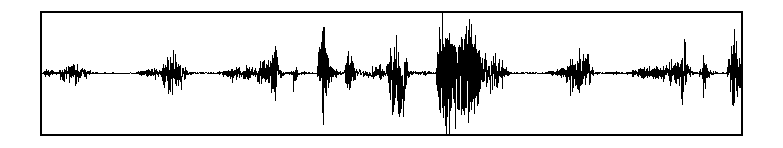
\epsfig{file=songwithSpect.eps,width=3in}  \\
{\large $\times 20$} \\
\vdots \\
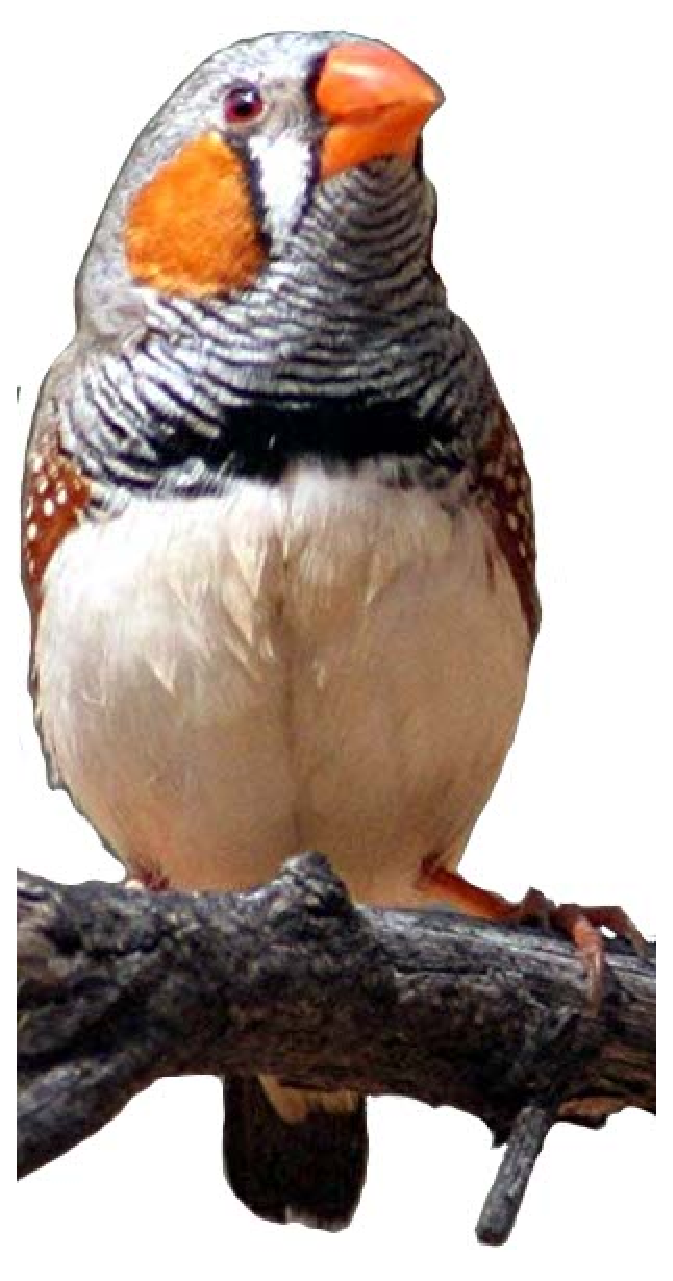
\epsfig{file=Finch-Zebra.eps,width=0.5in}\\ 
\vdots \\
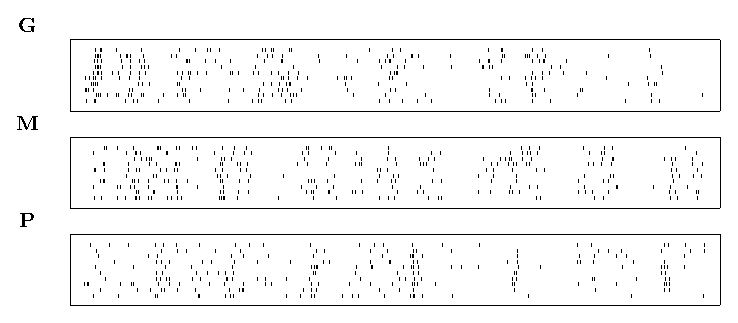
\epsfig{file=raster.eps,width=3in} 
\end{tabular}
\bigskip
\rule{33em}{0.5pt}
\caption{The data used was collected for \citep{NarayanEtAl2006b}.  A total of 20 songs were played to anaesthetised zebra finches, and the responses were recorded in the auditory forebrain.  Each song was presented ten times.  Responses for three different cells are shown here.}
\end{center}
\end{figure}

Zebra finch data is of particular use in Chapter Four, as there is evidence of feature recognition in responses to natural songs in the zebra finch forebrain \citep{SenEtAl2001a}.  Chapter Four introduces a simple model of firing which would be consistent with sparse coding.  Data sets with highly temporal features are thus important in testing the model.

\subsection{Multi-unit data}

\begin{figure}[htb]
\begin{center}
\setlength{\unitlength}{0.1cm}
\begin{picture}(110,90)
\put(30,10){\vector(0,1){6}}
\put(70,10){\vector(0,1){6}}
\put(30,16){\line(0,1){4}}
\put(70,16){\line(0,1){4}}
\put(30,25){\circle{10}}
\put(70,25){\circle{10}}
\put(78,26){\mbox{{\bf Receptive}}}
\put(78,21){\mbox{{\bf field neurons}}}
\put(30,30){\vector(0,1){11}}
\put(70,30){\vector(0,1){11}}
\put(30,41){\line(0,1){9}}
\put(70,41){\line(0,1){9}}

\put(30,30){\vector(2,1){26}}
\put(56,43){\line(2,1){14}}
\put(70,30){\vector(-2,1){26}}
\put(44,43){\line(-2,1){14}}
\put(30,55){\circle{10}}
\put(70,55){\circle{10}}
\put(78,56){\mbox{{\bf Integrate and}}}
\put(78,51){\mbox{{\bf fire neurons}}}
\put(80,39.5){\mbox{Poisson spiking}}
\put(80,34.5){\mbox{background}}
\put(0,40){\mbox{Poisson spiking}}
\put(0,35){\mbox{background}}
\put(16,43){\vector(2,1){10}}
\put(26,48){\line(2,1){4}}
\put(84,43){\vector(-2,1){10}}
\put(74,48){\line(-2,1){4}}

\put(32,39){\mbox{$a$}}
\put(72,39){\mbox{$a$}}
\put(22,4){\mbox{Stimuli (pairs of rate functions)}}
\put(22,72){\mbox{Responses (pairs of spike trains)}}

\put(70,66){\line(0,1){4}}
\put(30,60){\vector(0,1){6}}
\put(70,60){\vector(0,1){6}}
\put(30,66){\line(0,1){4}}
\put(46,45){\mbox{$1-a$}}
\end{picture}
\bigskip
\rule{33em}{0.5pt}
\end{center}
\caption{This is the schematic for the data set used to test the multi-unit metrics in this thesis.  It is the same data set that was used in \citep{HoughtonSen2008a}. The receptive field neurons fire Poisson spike trains according to the rate function input they receive. These Poisson spike trains feed into the leaky integrate and fire neurons from which the response is measured. The synaptic strengths are parametrised by $a$.  When $a$ is zero, the neurons receive independent input; when $a=0.5$, the input should be completely mixed. }
\end{figure}

The multi-unit distance measures  in chapter three were tested on the same simulated test data as in \citep{HoughtonSen2008a}. Two Poisson neurons form a receptive field and are each connected to two leaky integrate-and-fire neurons (LIF) with relative strength $a$ and $1-a$.  Hence, for $a=0$ each receptive neuron is connected to a single LIF neuron, and for $a=0.5$, each LIF neuron receives input equally from each of the receptive neurons.
 
The data consisted of five different stimuli, each presented 20 times, for a total of 100 responses.  These responses are clustered according to the bootstrapped procedure used in \citep{VictorPurpura1996a}. A confusion matrix is calculated whose entries $N_{ij}$ represent the number of responses from stimulus $i$ which are closest, on average, to the responses from stimulus $j$.


The transmitted information, $h$, is then calculated from the confusion matrix, $N$.
\begin{equation}
h = \frac{1}{n} \sum_{ij}N_{ij} \left( \ln N_{ij} - \ln \sum_i N_{ij} - \ln \sum_j N_{ij} + \ln n\right) .
\end{equation}
The transmitted information has maximum value $\ln(5)$, as there are five stimuli in this test.
 
While it may be preferable to test metrics on biological data in most cases, it is crucial to compare the performance of the multi-unit metrics with a controlled mixing parameter.  This test can then also compare how well a population parameter tunes a multi-unit metric by examining which parameter provided the maximum transmitted information for each mixing parameter.


